\documentclass{article}
\usepackage[utf8]{inputenc}
\usepackage{amsmath}
\usepackage{graphicx}
\usepackage{physics}
\usepackage{listings}
\begin{document}
\section{Problem 2 within project 1}
We are looking to write a program that defines a vector of x-values, and a function that evaluates the excact solution over these values, the results of which
will be stored in 2 columns, with a fixed amount of decimals, in scientific notation. This data will also be plotted  using a separate script.
\subsection*{The function}
we've implemented a function that returns a double $u(x)$ for an argument $x$, who's type is double, such that:
\begin{align}    
    \label{eq:excact_solution}
    u(x) =  1 - (1-e^{-10})x - e^{-10x}
\end{align}
x is a vector containing 101 linearly spaced doubles ranging from 0 to 1, and u is similarily a vector of doubles, such that $u_i=u(x_i)$. The elements of these vectors are stored in a .dat file,
and loaded using python, for which the data is used to initialize numpy arrays, for the purpose of displaying u(x). The results of which can be seen in the figure:
\begin{figure}[h]
    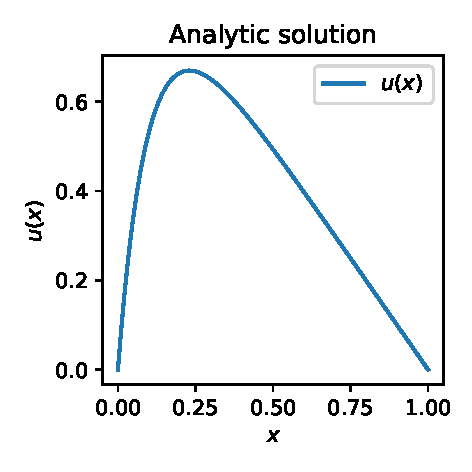
\includegraphics{problem_2_fig.pdf}
    \caption{Shows 101 linearly spaced points starting at 0 and ending at 1, evaluated on the excact solution $u(x)=1 - (1 - e^{-10})x - e^{-10x}$.}
\end{figure}
\end{document}